\section{Rear: Rear Exocentric Augmented Reality}
\label{sec:rear}

\subsection{How it works}
In this chapter we briefly describe how all the exocentric vision
is implemented, along with its business logic. In order to achieve
this, we will occasionally refer to the class diagram shown in figure
\ref{fig:class_diagram}.
%
\begin{figure}[!h]
  \begin{center}
    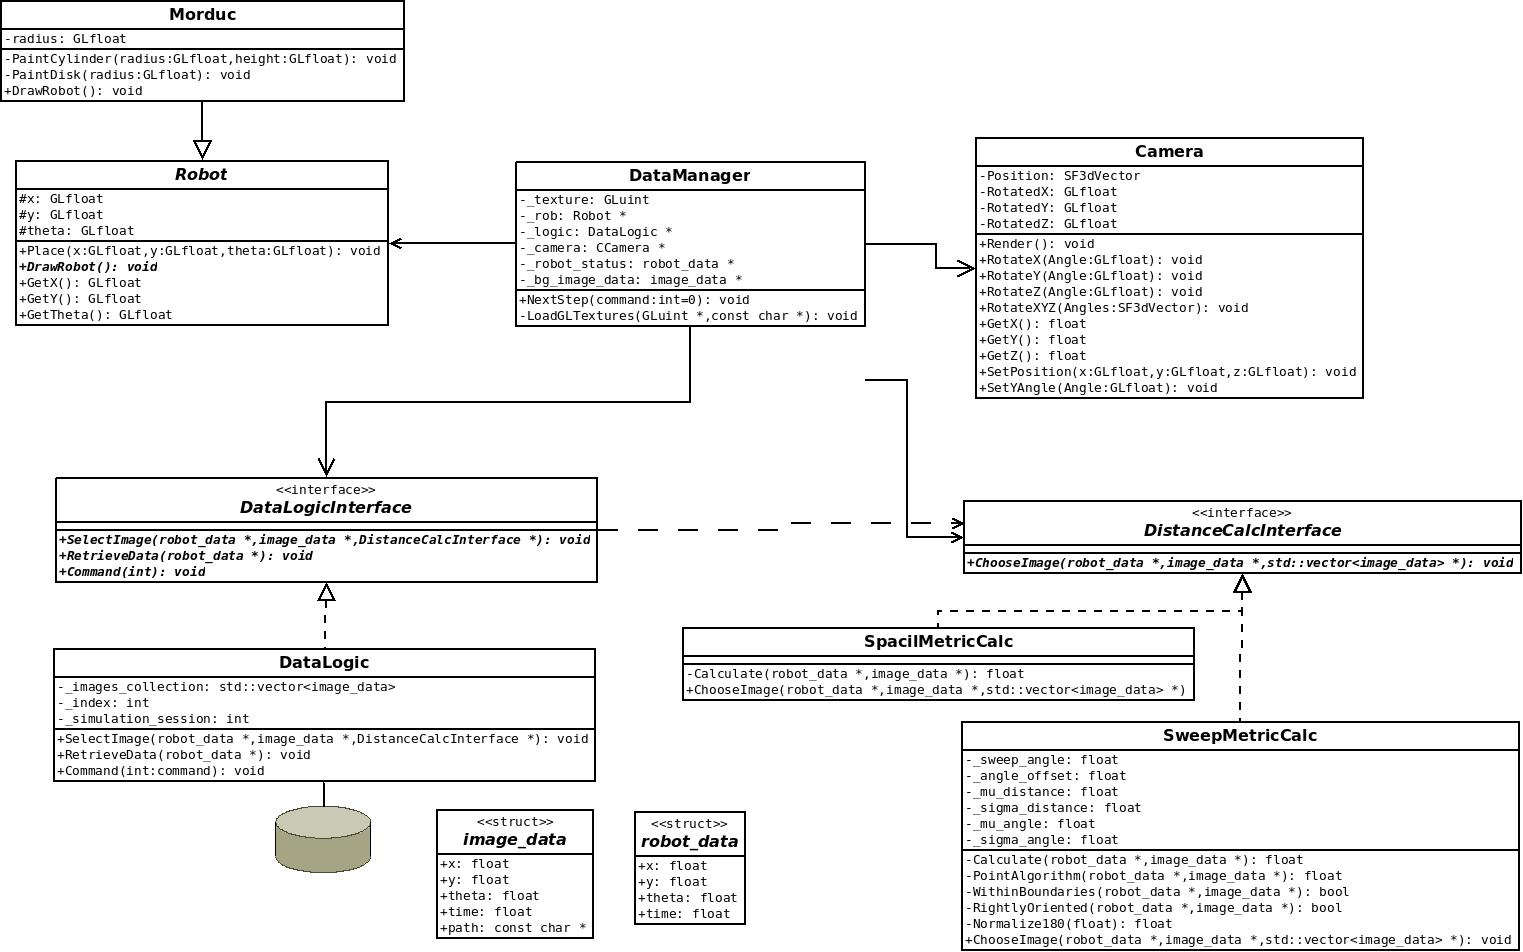
\includegraphics[width=400pt]{img/class_diagram.jpeg}  %robot pic
    \caption{Application class diagram}
    \label{fig:class_diagram}
  \end{center}
\end{figure}
%
The overall schema can be resumed by the following diagram (see figure
\ref{fig:overall_diagram}). User sends a command to the exocentric vision
application, in order to guide the robot through the remote environment.
The exocentric vision application forwards the command to the robot or the
simulator (paragraph \ref{sec:simulator}) and waits for the response.
The latter includes the new robot position and the new egocentric camera images.
%

%
All the egocentric camera images retrieved are stored in a data set and coupled
with robot coordinates and orientation at the moment when they were shot. Going
on with the application a large collection of egocentric images will be gathered.
%
\begin{figure}[!h]
  \begin{center}
    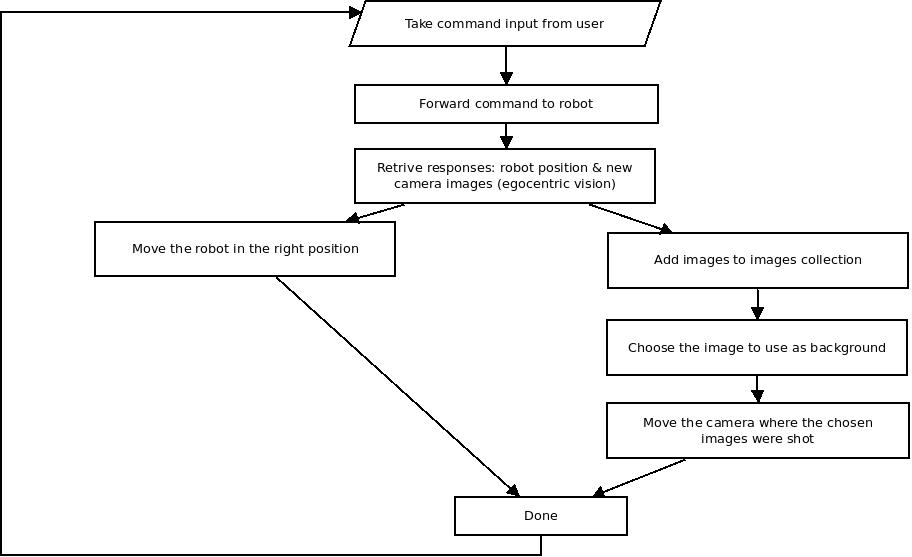
\includegraphics[width=400pt]{img/overall_diagram.jpeg}  %robot pic
    \caption{Application class diagram}
    \label{fig:overall_diagram}
  \end{center}
\end{figure}
%
After retrieving response from robot, the exocentric vision application moves the
robot in the openGL world (according to the robot coordinates read) and adds the
images received to the images collection. Later on, the application has to choose
the proper image (among those collected in the set) to use as texture (i.e. background)
in OpenGL and implement the exocentric vision.
%

%
Since every image owns its data about position and orientation when shot, we can
move and point the camera object to obtain the right visual of the external world.
Wherever the robot is situated, we will be able to watch it from the right point of view,
depending on the texture image chosen.
%

%
All the process explained above is lacking of one part: how to choose the background image,
knowing the actual robot position and orientation. If we decided to choose the closest image
to the robot we would always show the egocentric vision, because the algorithm would select
always the image with the same position and orientation of the robot. The distance between
the robot and the selected images would be equal to zero, which is doubtless the minimum possible
value.
%

%
The algorithms to take the right image in exocentric vision can be various. Each one has its own
advantages and disadvantages, we will chose the one able to guarantee the best trade-off.


\subsection{The Robot class}
The robot class, present in Filippo Privitera's simulator 
\cite{privitera}, has been simplified and then introduced in
exocentric vision control code. In this chapter we will 
exam the main differences.
%

%
Both classes represent the 3morduc robot in openGL world. 
This means that the robot class offers, among others, a
method with the purpose of drawing itself, called by the 
OpenGL framework when it is necessary. The operation of 
drawing is completed thanks to other two methods, able 
to draw the elementary part of the robot - e.g. cylinders and disks.
%

%
There are not considerable different between the tho 
drawing method implantation. The main one is that in the 
new method, before starting drawing, the model-view matrix 
is copied in order to restore it at the end of the process. 
In these way we do not affect the model-view matrix status 
by drawing the robot.
%

%
The robot class, after the refactoring process, loses many 
of its public attributes and methods, so in the
exocentric vision control it is much more simple than the 
original one. First of all, the new class does not contain either
attributes to store the actual speed vector component, or 
a chronometer object to count the time, or information about wheels
encoder. This information was stored in the simulator robot 
class to calculate the position of the robot after a movement,
but since we retrieve the position directly from the simulator 
these fields are now useless. 
%

%
The unique attribute (changed from public to private, in 
the new version) which survives the refactory - along with the
triple values indicating coordinate on x axis, coordinate on 
y axis and rotation - is named 'radius'. 'radius' is a float
attribute, which stores the value of the radius for the 
tree cylinders which make up the robot. See figure
\ref{fig:3morduc_opengl} for a better understanding.
%
\begin{figure}[!h]
  \begin{center}
    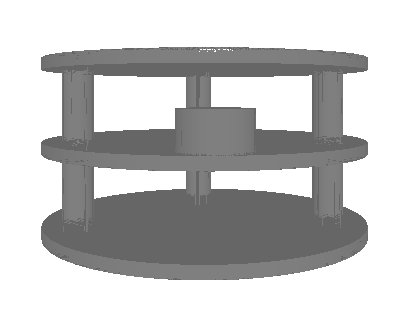
\includegraphics[width=200pt]{img/3morduc_opengl.png}  %robot pic
    \caption{The 3morduc robotic platform drawn in OpenGL}
    \label{fig:3morduc_opengl}
  \end{center}
\end{figure}
%
The default \textit{radius} value is 4, but it can be 
customised by the user: by increasing it the robot will be 
displayed larger and larger on the screen, and viceversa.
%

%
All the attributes are private in the new robot class, 
so a method to get each one value is declared. 
%

%
Most of the previous public methods have been removed too. 
The constructor method, for instance, is present with one
only definition and default parameters, instead of declaring 
it twice (with parameters and without). The methods to set
linear and angular velocity are not present anymore, for 
the reason explained above; those to increment the collisions 
number are actually disabled because, at this development 
stage, the exocentric vision control does not face the collision 
problem. Anyway, it is supposed to cope with collision in 
the future version.
%

%
Besides, the method used by Privitera's simulator to read 
the robot initial position from file has been removed, since 
for the exocentric vision system robot always starts from 
fixed coordinates and rotation.
%

%
Finally, the method named with the signature 
\begin{verbatim} 
void move() 
\end{verbatim} 
has been changed in 
\begin{verbatim} 
void Place(float x, float y, float theta)
\end{verbatim}
in order to set the x and y coordinate and the rotation of the robot. 
We remind that in the previous version these attributes
were public, so there were no need to pass them as parameters function.

\subsection{The Camera class}
First of all, there is no thing like a camera in OpenGL, therefore we have to
simulate one.
%

%
A camera object allows to move and rotate the user point of view and robot
object independently, avoiding that one interferes the other. For the exocentric
vision application this is a basic feature, because robot can be placed
everywhere in OpenGL world regardless of the camera position, and viceversa.
%

%
The camera object implementation has been suggested by \cite{opengl:camera}.
It provides some elementary commands implemented by means of mathematical matrix
operations, to move the camera or rotate it along one axis.
